\documentclass[journal,10pt,twocolumn]{article}
\usepackage[margin=0.5in]{geometry}
\usepackage[cmex10]{amsmath}
\usepackage{amsmath}
\usepackage{array}
\usepackage{booktabs}
% The preceding line is only needed to identify funding in the first footnote. If that is unneeded, please comment it out.
\usepackage{cite}
\usepackage{amsmath,amssymb,amsfonts}
\usepackage{graphicx}
\usepackage{textcomp}
\usepackage{xcolor}
\usepackage{graphicx}
\graphicspath{{./fig}}{}
\def\BibTeX{{\rm B\kern-.05em{\sc i\kern-.025em b}\kern-.08em
    T\kern-.1667em\lower.7ex\hbox{E}\kern-.125emX}}
\usepackage{tikz}
\usetikzlibrary{shapes.geometric}
\usetikzlibrary{shapes.geometric,angles,quotes}
\usepackage{mathtools}  
\usepackage{diffcoeff}  

\begin{document}
\newtheorem{theorem}{Theorem}[section]
\newtheorem{problem}{Problem}
\newtheorem{proposition}{Proposition}[section]
\newtheorem{lemma}{Lemma}[section]
\newtheorem{corollary}[theorem]{Corollary}
\newtheorem{example}{Example}[section]
\newtheorem{definition}[problem]{Definition}
%\newtheorem{thm}{Theorem}[section] 
%\newtheorem{defn}[thm]{Definition}
%\newtheorem{algorithm}{Algorithm}[section]
%\newtheorem{cor}{Corollary}
\newcommand{\BEQA}{\begin{eqnarray}}
\newcommand{\EEQA}{\end{eqnarray}}
\newcommand{\define}{\stackrel{\triangle}{=}}
\newcommand*\circled[1]{\tikz[baseline=(char.base)]{
    \node[shape=circle,draw,inner sep=2pt] (char) {#1};}}
\bibliographystyle{article}
%\bibliographystyle{ieeetr}
\providecommand{\mbf}{\mathbf}
\providecommand{\pr}[1]{\ensuremath{\Pr\left(#1\right)}}
\providecommand{\re}[1]{\ensuremath{\text{Re}\left(#1\right)}}
\providecommand{\im}[1]{\ensuremath{\text{Im}\left(#1\right)}}
\providecommand{\qfunc}[1]{\ensuremath{Q\left(#1\right)}}
\providecommand{\sbrak}[1]{\ensuremath{{}\left[#1\right]}}
\providecommand{\lsbrak}[1]{\ensuremath{{}\left[#1\right.}}
\providecommand{\rsbrak}[1]{\ensuremath{{}\left.#1\right]}}
\providecommand{\brak}[1]{\ensuremath{\left(#1\right)}}
\providecommand{\lbrak}[1]{\ensuremath{\left(#1\right.}}
\providecommand{\rbrak}[1]{\ensuremath{\left.#1\right)}}
\providecommand{\cbrak}[1]{\ensuremath{\left\{#1\right\}}}
\providecommand{\lcbrak}[1]{\ensuremath{\left\{#1\right.}}
\providecommand{\rcbrak}[1]{\ensuremath{\left.#1\right\}}}
\newcommand{\sgn}{\mathop{\mathrm{sgn}}}
%\providecommand{\hilbert}{\overset{\mathcal{H}}{ \rightleftharpoons}}
\providecommand{\system}{\overset{\mathcal{H}}{ \longleftrightarrow}}
	%\newcommand{\solution}[2]{\textbf{Solution:}{#1}}
\newcommand{\solution}{\noindent \textbf{Solution: }}
\newcommand{\cosec}{\,\text{cosec}\,}
\providecommand{\dec}[2]{\ensuremath{\overset{#1}{\underset{#2}{\gtrless}}}}
\newcommand{\myvec}[1]{\ensuremath{\begin{pmatrix}#1\end{pmatrix}}}
\newcommand{\mydet}[1]{\ensuremath{\begin{vmatrix}#1\end{vmatrix}}}
	\newcommand*{\permcomb}[4][0mu]{{{}^{#3}\mkern#1#2_{#4}}}
\newcommand*{\perm}[1][-3mu]{\permcomb[#1]{P}}
\newcommand*{\comb}[1][-1mu]{\permcomb[#1]{C}}
%\numberwithin{equation}{section}
\numberwithin{equation}{subsection}
%\numberwithin{problem}{section}
%\numberwithin{definition}{section}
\let\vec\mathbf
\title{
{Verification of Distributive Laws of Boolean Algebra \\
Using ARM Processor-VAMAN Board}\\
\thanks {Meer Tabres Ali as an intern with FWC IIT Hyderabad. *The author is with the Department of Electrical Engineering, Indian Institute of Technology, Hyderabad 502285 India e-mail: gadepall@iith.ac.in. All content in this manual is released under GNU GPL. Free and open source.}
}
\author{Meer Tabres Ali and G V V Sharma}
\maketitle
\tableofcontents
\section{Problem statement}
\begin{flushleft}
Verification of \textbf{Distributive Law}of Boolean Algebra using\\
\vspace{0.25cm}
\textbf{ARM} Processor-\textbf{VAMAN} Board\\
\end{flushleft}
\section{Abstract}
\begin{flushleft}
Distributive laws of Boolean Algebra is expressed by the following expression.\\
\vspace{0.25cm}
Distributive Law: \textbf{X.(Y+Z) = X.Y + X.Z} \\
\vspace{0.25cm}

In this program, Two LEDs are used for checking the output. The outputs of both RHS and LHS parts of above expression must be same with the random inputs.\\
\end{flushleft}

\section{Truth Table for Distributive Laws}
Truth Table for Distributive Law: X.(Y+Z) = X.Y + X.Z 

\begin{table}[htbp]
    \centering
\begin{tabular}{ | c | c | c | c | c | c | c | c | } \hline
\textbf{X} & \textbf{Y} & \textbf{Z} & Y+Z & \textbf{X(Y+Z)} & XY & XZ & \textbf{XY+XZ} \\\hline
0 & 0 & 0 & 0 & 0 & 0 & 0 & 0 \\
0 & 0 & 1 & 0 & 0 & 0 & 0 & 0 \\
0 & 1 & 0 & 0 & 0 & 0 & 0 & 0 \\
0 & 1 & 1 & 0 & 0 & 0 & 0 & 0 \\
1 & 0 & 0 & 0 & 0 & 0 & 0 & 0 \\
1 & 0 & 1 & 1 & 1 & 0 & 1 & 1 \\
1 & 1 & 0 & 1 & 1 & 1 & 0 & 1 \\
1 & 1 & 1 & 1 & 1 & 1 & 1 & 1 \\ \hline
\end{tabular}
\caption{\label{tab:widgets}Truth Table for Distributive Law1}
\end{table}
\section{Considerations}
\vspace{0.2cm}
\begin{flushleft}
As per given data, the following table has been prepared.\\
\end{flushleft}
\vspace{0.3cm}
\begin{table}[htbp]
    \centering
\setlength\extrarowheight{2pt}
\begin{tabular}{|c|c|c|} \hline
      \textbf{Symbol/Device}           &   \textbf{Value}   & \textbf{Description}\\ \hline
	\textbf{X, Y, Z }& Pin 2, 4, 6 & Input Variables\\  \hline
	\textbf{A,B} & Pin 18, 21 & Output Variables\\ \hline
	\textbf{VAMAN Board} &  1 & \\ \hline
    LEDs & 2 & For Output \\ \hline
 Connecting wires & 10 & For Output \\ \hline
\end{tabular}
\caption{\label{tab:widgets}Considerations}
\end{table}

\section{Logic diagram of gates}
\vspace{0.25cm}
Logic diagram of gates is shown in the figure 1.
\begin{figure}[h]
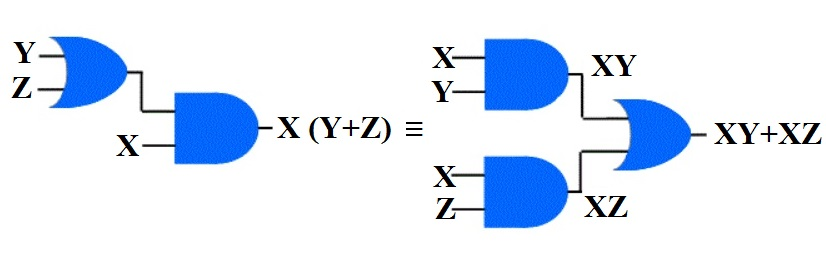
\includegraphics[width=1\columnwidth]{Gates.jpg}
\caption{Logic diagram of gates}
\label{Logic diagram of gates}
\end{figure}
\section{Solution}
\begin{flushleft}
1. Apply the inputs X, Y, and Z (either HIGH or LOW) to the  Pin no.s 2, 4 and 6 of \textbf{Vaman Board(Pigmy side)} as per the Truth tables.\\
2. Randomly vary the inputs and note the the results.
\end{flushleft}
\section{SOFTWARE}
\centering
1. Download the codes given in the link below and execute them.\\

\begin{table}[h]
\centering
\begin{tabular}{| c |} \hline
 \rule{0pt}{20pt} https://github.com/meertabresali-FWC-IITH/project/blob/main/\\
 Asgn9.Arm/codes/src/main.c \\\hline
\end{tabular}
\end{table}



\section{CONCLUSION}
\begin{flushleft}
1. Distributive law is expressed by \\
\vspace{0.25cm}
X(Y+Z)=XY+XZ with LHS = X(Y+Z), RHS = XY+XZ, and \\
\vspace{0.25cm}
2. Codes are written for both Distributive laws and are executed using Vaman Board(Arm processor).\\
3. Result has been displayed on LEDs (i.e. LED1, LED2). \\
4. LED1 is assigned for LHS of the Boolean expression of Distributive Law. \\
5. LED2 is assigned for RHS of the Boolean expression of Distributive Law. \\
6. For random digital inputs X, Y and Z as per Truth tables (at Vaman Board(Pigmy side)  pins 2, 4 and 6), it has been noticed that, the output pins (18 and 21) of Vaman Board are at the same level.\\

\end{flushleft}
\end{document}
